
\chapter{Methods}
The present chapter provides an outline of the methodology employed to automate the documentation process. The subsequent sections present a detailed description of the project setup within and between the teams from Chalmers and Penn State University, outlining how the information was gathered, and the methods utilized to validate the final product at the end of the project.

\section{Project setup and structure}
The team consisted of students from both Chalmers University of Technology
and Penn State University. There were six students from Chalmers with majors in Mechanical Engineering, and Automation and Mechatronics, with three students in each major. There were also six students from Penn State with diverse majors, Mechanical Engineering (3), Computer Science (1), and Computer Engineering (2). This diversification in educational foundation provided complementing strengths that were applied during the project.
\\

The primary objective for the Chalmers team was to develop an Android application. Said application would facilitate communication between the drone and the control system (ATOS), both supplied by AstaZero. However, the ATOS software lacked the capability to calculate drone trajectories and needed to be implemented. As outlined in Sec.~\ref{AZ's app}, AstaZero had already developed an Android application with limited functionality with basic features that allowed communication with the drone. The objective was to keep developing this application to give it more features and automate it. The project's main objective was software development and did not involve any physical construction, as outlined in Sec.~\ref{chap:problem statement}.
% Documentation and report writing was done continuously thought all phases of the project, see Sec.~\ref{chap:problem statement}. To keep track of all the different tasks and what tasks were assigned to whom, the application Trello~\cite{AtlassianTrello} was used as a project management board. Within the project, different persons had different roles. Some were project managers, responsible for the reports, administration, Trello board, and deadlines, and some focused more on developing the application. Fig. ~\ref{fig:workflow} shows how the work was divided into different phases of the project.

% \begin{figure}[H]
%   \centering
%   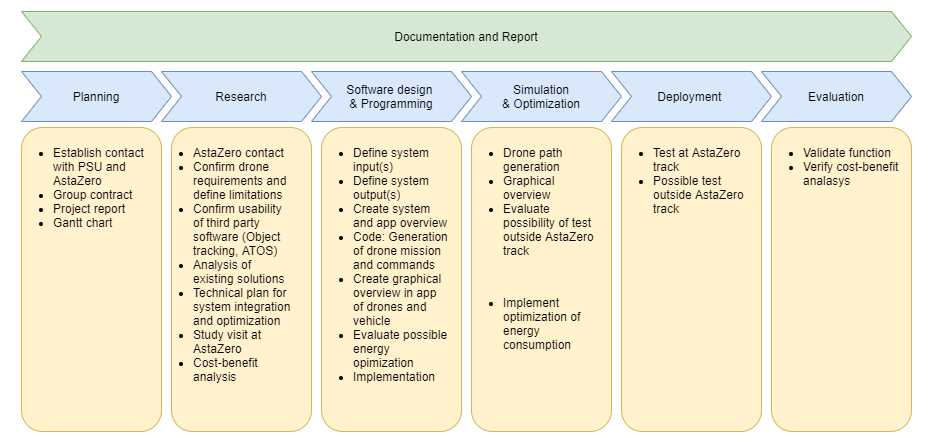
\includegraphics[width=\columnwidth]{figure/work_flow.png}
%   \caption{Work flow of the project. Source: Primary}
%   \label{fig:workflow}
% \end{figure}

\subsection{Work distribution between the two universities}
As previously stated, the Bachelor's Thesis work was conducted as a joint venture between Chalmers and PSU. Due to the time difference between the two universities, it was crucial to clearly define the division of labor. This facilitated consistent and independent work from each group, eliminating the need for constant communication.
\\ \\
For the configuration to function properly, two pieces of software needed to be developed and integrated: ATOS and the drone application. This setup allowed for a natural division of labor between the universities, as both the application and ATOS, which had already been developed by AstaZero, could be worked on independently.
\\ \\
Accordingly, the Chalmers team was solely responsible for developing the drone application, while the PSU team handled the orchestration of the test objects (ATOS) and path calculations. However, since both ATOS and the application were equally crucial for the success of the project, and equally crucial for the configuration to even operate, both groups had to be held accountable for upholding their part of the project. A more descriptive view over the distribution can be seen in Fig.~\ref{fig:DividedBetweenUni} below, where AZ is short for AstaZero.

\begin{figure}[H]
  \centering
  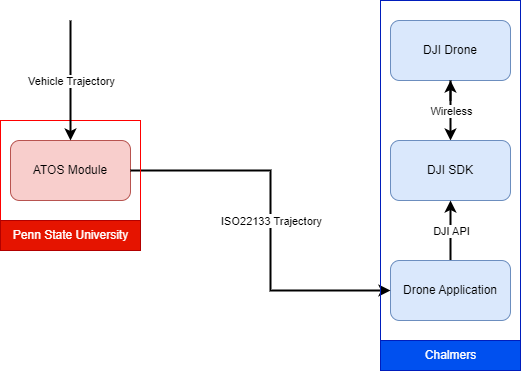
\includegraphics[width=0.7\textwidth]{figure/work distribution.png}
  \caption{Illustration of the work distribution between the universities. Source: Primary}
  \label{fig:DividedBetweenUni}
\end{figure}

PSU were tasked with determining the precise flight trajectory, dictating the drone's specific positioning at designated times, commonly referred to as trajectories.
According to ISO22133~\cite{iso22133}, trajectories are a collection of waypoints to define a path of a single test object during test, added by a time  stamp  for  each  waypoint (location  and  time) and test-object dynamics   (e.g.   yaw,   velocity,   acceleration). In line with Sec.~\ref{sec:project outline} of the project outline, PSU are responsible for providing the accurate trajectory required to capture footage at the appropriate zoom level and angle. Hence, the primary task of the Chalmers team entails enabling the drone to precisely navigate its designated trajectory, while  tracing the car with the drone's camera.


% \section{Scoping and information gathering}
% Research and information gathering was conducted continuously throughout the project and encompassed the majority of the project's initial workload. The research commenced with the introduction given by Victor Jarlow, the point of contact at AstaZero. This presentation gave crucial information on how a Euro NCAP trial was performed at the test site, how ATOS worked, as well as the project's parameters and goals.
% \\ \\
% Knowledge was consequently gathered of what AstaZero already had produced and what was relevant to integrate into a new application. Since the existing application also used the same communication protocol, gathering a deep understanding of the code was beneficial for the continued development of the application. The application is not intended for commercial use and was therefore not well documented, accordingly, understanding the already existing code was done by reading and testing.
\section{Test driven development}
Throughout the project, the software development methodology known as Test-Driven Development (TDD)~\cite{TestDriven.ioWhatDevelopment} was a source of inspiration. TDD is a process that follows an iterative development cycle and involves the creation of tests before writing the code itself. As a component of the agile software development approach, TDD emphasizes continuous integration, testing, and deployment.
\\

In order to ensure the robustness of each subsystem of the drone application, it was crucial to continuously test them. This approach helped to facilitate a smoother integration process, while also providing ease in identifying any subsystem failures. TDD is based on five fundamental steps which is detalied in the following list and Fig.~\ref{fig:TDD}:
\vspace{0.2cm}
\begin{enumerate}
    \item Think of what the next step of the code development is. Thereafter, add a test pertaining to the problem at hand, as detailed as possible.
    \item Do not write any code which purpose is to solve the issue, i.e ensure that the test fails. The test failure provides insight in what needs to be done.
    \item Write new code which purpose is to pass the test. 
    \item Ensure that the test succeeds
    \item Refactor the code, i.e make it more efficient without altering functionality
\end{enumerate}
\begin{figure}[H]
  \centering
  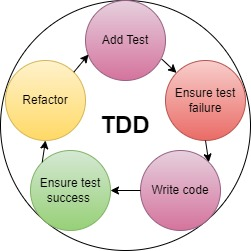
\includegraphics[width=0.5\textwidth]{figure/TDD.jpg}
  \caption{Illustration of test driven development. Source: Primary}
  \label{fig:TDD}
\end{figure}
Throughout the project, the application of TDD has proved to be highly advantageous in the development of the application, with a specifying predefined goal for each function. However, there are some major disparities between the development method applied in the project and TDD. Instead of actually writing tests in the code, actual physical tests were conducted for each improvement of the code. Since the software development concerns drone flight and camera-gimbal movement, ensuring that a test fails is, needless to say, not a great idea. Nevertheless, TDD's modular approach to code development and ease for step-by-step improvement was of immense help and contributed to making the code easier to maintain. 

% \section{Code development}

% The major challenges of the project were deemed to be object detection and controlling the drone's flight in accordance with the desired trajectory. The two problems were worked on in parallel with a goal of merging them once they were independently fully functional. 
% \\ \\
% Research went into existing pre-trained object detection model, as opposed to developing one from scratch. While there was some previous experience with image classification and CNNs, there was no prior experience with object detection. Object detection presents additional challenges beyond image classification, as it cannot be assumed that objects are centered in the input image, and multiple objects may be present. Creating and training a custom model to address these complexities, would have been too time-consuming, given that efficient and accurate pre-trained models already exist. 
% \\ \\
% As previously mentioned, the code that handled the flight of the drone was based on the DJI demo application provided by AstaZero as outlined in Sec.~\ref{AZ's app} and the DJI WaypointMission. Since the provided application already connects to the drone, the goal of the new application was to integrate flight control with the ATOS module.

\section{Validation}
\label{sec:val}
Validation assessments were conducted on various implementations of the application, with a specific focus on flight control and object detection. The results of these assessments formed the basis for the project outcomes and the ultimate demonstration at AstaZero's test track.

\subsection{Flight control}
\label{sec:val_flight}
To ensure that the application lived up to the wishes and demands from AstaZero, the drone and ATOS was extensively used in testing component implementations during the project, utilizing the TDD philosophy. The validation tests also laid ground for the results of the project and a demonstration scheduled to take place at AstaZero's test track.
\\ \\
The same baseline for the majority of the tests conducted regarding flight control and WaypointMission. In the ATOS program, a virtual road with the length of 25 m was set up with an origin at a specific spot, chosen in longitudinal and latitudinal coordinates within ATOS. The complexity of the test was then gradually increased to see how different parts worked together. The following list showcases the most important tests conducted:
\\
\begin{itemize}\itemsep0.2em
    \item Achieve automatic takeoff and landing without ATOS control
    \item Achieve automatic takeoff and landing with ATOS control
    \item Run predetermined WaypointMission from application without ATOS control
    \item Run predetermined WaypointMission from application with ATOS control
    \item Generate trajectory in ATOS, convert it to WaypointMission and run test with ATOS control.\\
\end{itemize}

To ensure that the drone would not pose any danger to anyone, the EmergencyStop function was thoroughly tested with multiple different scenarios. Tests were conducted where the EmergencyStop was issued from both the GUI and the ATOS program in different states of the mission such as the uploading and running phases. To prevent any damage, the EmergencyStop function only stops the drone and the operators had to land the drone manually.

\subsection{Object detection}
\label{val_obj_det}
In order to ascertain whether the model was suitable for the project, tests were conducted to ensure desirable object detection performance. Given the limited prior experience in object detection, fundamental tests were set up to ensure gradual and steady progress in development. As object detection with a mobile device is a well-documented area, the initial development and testing was done with a camera on a mobile device. The tests were the following:
\\
\begin{itemize}\itemsep0.2em
    \item Setting up the model on the supplied mobile device
    \item Film non moving objects
    \item Film moving cars and persons
    \item Test model output frequency \\
\end{itemize}

Concurrently, a test was conducted on the drone to prepare for the integration of object detection. As the application solely retrieves the position of the selected object, it was necessary to confirm whether the camera angle could be adjusted during a WaypointMission. The test demonstrated that it was feasible to adjust the drone's gimbal while simultaneously executing a WaypointMission.
